\documentclass[12pt,a4paper]{report}

% ── Packages ──────────────────────────────────────────────────────────────────
\usepackage[a4paper, margin=2.5cm, top=3cm, bottom=3cm]{geometry}
\usepackage[T1]{fontenc}
\usepackage[utf8]{inputenc}
\usepackage{graphicx}
\usepackage{booktabs}
\usepackage{array}
\usepackage{tabularx}
\usepackage[table]{xcolor}
\usepackage{enumitem}
\usepackage{parskip}
\usepackage{titlesec}
\usepackage{fancyhdr}
\usepackage{hyperref}
\usepackage{tcolorbox}
\usepackage{amsmath}
\usepackage{caption}
\usepackage[nottoc]{tocbibind}

% ── Colours ───────────────────────────────────────────────────────────────────
\definecolor{darkblue}{HTML}{1F4E79}
\definecolor{medblue}{HTML}{2E74B5}
\definecolor{lightblue}{HTML}{D6E4F0}
\definecolor{altrow}{HTML}{EBF3FB}
\definecolor{greenbg}{HTML}{E2EFDA}
\definecolor{headerbg}{HTML}{1F4E79}
\definecolor{statusgreen}{HTML}{70AD47}
\definecolor{statusamber}{HTML}{FFC000}

% ── tcolorbox ─────────────────────────────────────────────────────────────────
\tcbuselibrary{skins, breakable}

\newtcolorbox{deliverablebox}[1]{
  colback=greenbg, colframe=darkblue, coltitle=white,
  fonttitle=\bfseries, title={#1},
  breakable, boxrule=0.8pt, arc=3pt,
  left=6pt, right=6pt, top=4pt, bottom=4pt
}
\newtcolorbox{infobox}{
  colback=lightblue!60, colframe=medblue,
  boxrule=0.6pt, arc=2pt,
  left=6pt, right=6pt, top=3pt, bottom=3pt
}

% ── Caption style ─────────────────────────────────────────────────────────────
\captionsetup{font=small, labelfont=bf, labelsep=period}

% ── Section formatting ────────────────────────────────────────────────────────
\titleformat{\chapter}[block]
  {\Large\bfseries\color{darkblue}}{\thechapter.}{0.6em}{}
  [\color{medblue}\titlerule]
\titleformat{\section}[block]
  {\large\bfseries\color{medblue}}{\thesection}{0.5em}{}
\titleformat{\subsection}[block]
  {\normalsize\bfseries\color{darkblue!80}}{\thesubsection}{0.5em}{}
\titlespacing*{\chapter}{0pt}{12pt}{10pt}
\titlespacing*{\section}{0pt}{10pt}{6pt}
\titlespacing*{\subsection}{0pt}{8pt}{4pt}

% ── Header / Footer ───────────────────────────────────────────────────────────
\pagestyle{fancy}
\fancyhf{}
\renewcommand{\headrulewidth}{0.4pt}
\renewcommand{\footrulewidth}{0.4pt}
\fancyhead[L]{\small\color{darkblue}\textbf{Phase 2 Completion Report}}
\fancyhead[R]{\small\color{darkblue}Rajib Roy --- 24459 $|$ IISc M.Tech (AI)}
\fancyfoot[C]{\small\thepage}
\fancyfoot[R]{\small\color{gray}July 2026}

% ── Hyperref ──────────────────────────────────────────────────────────────────
\hypersetup{colorlinks=true, linkcolor=medblue, urlcolor=medblue,
  pdftitle={Phase 2 Completion Report --- Rajib Roy}, pdfauthor={Rajib Roy}}

% ── Table column types ────────────────────────────────────────────────────────
\newcolumntype{L}[1]{>{\raggedright\arraybackslash}p{#1}}
\newcolumntype{C}[1]{>{\centering\arraybackslash}p{#1}}

% ── Status macros ─────────────────────────────────────────────────────────────
\newcommand{\statuscomplete}{\colorbox{statusgreen}{\color{white}\textbf{\small Complete}}}
\newcommand{\statusphase}[1]{\colorbox{statusamber}{\color{white}\textbf{\small #1}}}

% ── Lists ─────────────────────────────────────────────────────────────────────
\setlist[itemize]{leftmargin=1.4em, itemsep=3pt, topsep=4pt}
\setlist[enumerate]{leftmargin=1.4em, itemsep=3pt, topsep=4pt}

% ── Graphics path ─────────────────────────────────────────────────────────────
\graphicspath{{./}}

% ═════════════════════════════════════════════════════════════════════════════
\begin{document}
\pagenumbering{roman}

% ── COVER PAGE ────────────────────────────────────────────────────────────────
\begin{titlepage}
  \thispagestyle{empty}
  \begin{center}
    \vspace*{1cm}
    {\large\color{darkblue}M.Tech.\ (Online) --- Artificial Intelligence}\\[4pt]
    {\large\color{darkblue}Indian Institute of Science, Bangalore}\\[2cm]
    {\Huge\bfseries\color{darkblue}PHASE 2 COMPLETION REPORT}\\[1cm]
    {\color{medblue}\rule{\linewidth}{2pt}}\\[0.5cm]
    {\LARGE\bfseries\color{medblue}
      Detection of AI-Generated and Cloned Speech\\[6pt]
      to Strengthen Voice-Based Authentication\\[6pt]
      in Banking Environments}\\[0.4cm]
    {\color{medblue}\rule{\linewidth}{1pt}}\\[1.8cm]
    \begin{tabular}{@{}L{4.5cm}L{9cm}@{}}
      \rowcolor{lightblue}\textbf{Student Name}   & Rajib Roy \\
      \rowcolor{white}    \textbf{Student Number} & 24459 \\
      \rowcolor{lightblue}\textbf{Programme}      & M.Tech.\ in Artificial Intelligence \\
      \rowcolor{white}    \textbf{Internal Guide} & Dr.\ Anil Rahate, Practice Head --- AI, Wipro Ltd \\
      \rowcolor{lightblue}\textbf{IISc Mentor}    & Prof.\ Chandra Sekhar Seelamantula,
                                                     Dept.\ of Electrical Engineering, IISc \\
      \rowcolor{white}    \textbf{Phase Covered}  & Phase 2 \quad (May 2026 --- July 2026) \\
      \rowcolor{lightblue}\textbf{Report Date}    & July 2026 \\
    \end{tabular}
  \end{center}
\end{titlepage}

\tableofcontents
\listoffigures
\clearpage
\pagenumbering{arabic}

% ═════════════════════════════════════════════════════════════════════════════
\chapter{Executive Summary}
% ═════════════════════════════════════════════════════════════════════════════

This report documents the completion of \textbf{Phase 2} of the M.Tech.\ project titled
\textit{Detection of AI-Generated and Cloned Speech to Strengthen Voice-Based Authentication
in Banking Environments}. Phase 2 is scoped against the \textbf{Revised Plan for Phase 2}
set out at the end of the Phase 1 Completion Report --- the explicit commitment made to the
internal guide and IISc faculty mentor at the close of Phase 1 --- rather than a re-reading of
the original proposal's phase boundaries. That revised plan lists four technical deliverables:
classical machine learning baselines, feature importance analysis, deep learning model
development (CNN, CNN-LSTM), and robustness experiments across noise and codec conditions,
plus this written interim report.

\textbf{All four technical deliverables have been completed on schedule}, building directly
on the 17{,}947-utterance dataset and 257-dimensional feature pipeline validated in Phase 1.

\medskip
\begin{center}
\begin{tabular}{L{4.2cm}L{6.8cm}C{2cm}}
  \toprule
  \rowcolor{headerbg}
  \color{white}\textbf{Deliverable} &
  \color{white}\textbf{Outcome} &
  \color{white}\textbf{Status} \\
  \midrule
  Classical ML baselines (SVM, RF, Gradient Boosting) &
  SVM best classical model: EER 0.0083, F1 0.9943 on standard test set; all three
  models generalise well to held-out Edge-TTS &
  \statuscomplete \\[4pt]
  \rowcolor{altrow}
  Feature importance analysis &
  Random Forest importances identify delta-MFCC coefficients as the dominant
  discriminators, validating the Phase 1 feature design &
  \statuscomplete \\[4pt]
  Deep learning models (CNN, CNN-LSTM) &
  CNN-LSTM is the best model overall: EER 0.0035 on test, EER 0.0004 on
  generalisation test (AUC $=1.000$) &
  \statuscomplete \\[4pt]
  \rowcolor{altrow}
  Robustness \& generalisation evaluation &
  Degradation curves across SNR (5--20\,dB) and G.711 codec; every model
  generalises to unseen Edge-TTS as well as or better than on the standard test &
  \statuscomplete \\
  \bottomrule
\end{tabular}
\end{center}

\medskip
The headline result is that the \textbf{CNN-LSTM} achieves an Equal Error Rate (EER) of
\textbf{0.0035} on the standard test set and an almost perfect EER of \textbf{0.0004} on the
fully held-out Microsoft Edge-TTS generalisation set --- a TTS system never seen during
training. The SVM baseline, using only handcrafted acoustic features, is a strong and
computationally cheap alternative (EER 0.0083), confirming the Phase 1 literature-driven
feature design. Robustness testing shows that additive noise is a substantially more severe
deployment threat than G.711 codec compression, directly informing the Phase 3 hardening
plan.

% ═════════════════════════════════════════════════════════════════════════════
\chapter{Phase 2 Deliverables in Detail}
% ═════════════════════════════════════════════════════════════════════════════

% ─────────────────────────────────────────────────────────────────────────────
\section{Classical Machine Learning Baselines}
% ─────────────────────────────────────────────────────────────────────────────

\textbf{Objective:} Train and tune SVM, Random Forest, and Gradient Boosting classifiers on
the 257-dimensional handcrafted feature vectors from Phase 1, establishing reproducible
baselines against which the deep learning models are compared.

\subsection{Training Protocol}

All three classifiers (\texttt{03\_train\_baselines.py}) were trained with
\texttt{class\_weight=`balanced'} and SMOTE oversampling inside stratified 5-fold
cross-validation grid search, using ROC-AUC as the optimisation objective. Decision
thresholds were fixed at the EER operating point measured on the validation split.
Selected hyperparameters: SVM (RBF kernel, $C=10$, $\gamma=\text{auto}$); Random Forest
(300 estimators, unlimited depth); Gradient Boosting (200 estimators, learning rate 0.1).

\subsection{Baseline Results}

\begin{center}
\begin{tabular}{L{3cm}L{2.6cm}C{1.5cm}C{1.3cm}C{1.3cm}C{1.4cm}}
  \toprule
  \rowcolor{headerbg}
  \color{white}\textbf{Model} &
  \color{white}\textbf{Eval.\ Set} &
  \color{white}\textbf{EER $\downarrow$} &
  \color{white}\textbf{F1 $\uparrow$} &
  \color{white}\textbf{AUC $\uparrow$} &
  \color{white}\textbf{Acc.\ $\uparrow$} \\
  \midrule
  SVM (RBF) & Test & 0.0083 & 0.9943 & 0.9992 & 0.9912 \\
  \rowcolor{altrow}
  SVM (RBF) & Gen.\ test$^\dagger$ & 0.0067 & 0.9969 & 0.9987 & 0.9953 \\
  Random Forest & Test & 0.0305 & 0.9834 & 0.9956 & 0.9744 \\
  \rowcolor{altrow}
  Random Forest & Gen.\ test$^\dagger$ & 0.0293 & 0.9854 & 0.9964 & 0.9781 \\
  Gradient Boosting & Test & 0.0346 & 0.9820 & 0.9949 & 0.9722 \\
  \rowcolor{altrow}
  Gradient Boosting & Gen.\ test$^\dagger$ & 0.0311 & 0.9868 & 0.9956 & 0.9801 \\
  \bottomrule
\end{tabular}
\captionof{table}{Classical baseline performance. $^\dagger$Gen.\ test = held-out Edge-TTS
(unseen during training).}
\label{tab:baselines}
\end{center}

\medskip
The SVM is the strongest classical model by a clear margin, and --- notably --- all three
classical models achieve \emph{equal or lower} EER on the unseen Edge-TTS generalisation set
than on the standard (in-distribution) test set. This indicates that the handcrafted
features capture TTS-system-agnostic artefacts rather than overfitting to the specific
synthesis systems seen in training.

\begin{deliverablebox}{Deliverable 1 --- COMPLETE}
  Three classical classifiers trained, tuned via 5-fold cross-validated grid search, and
  evaluated on both the standard test set and the held-out Edge-TTS generalisation set.
  SVM is established as the strongest and most efficient classical baseline
  (EER 0.0083), saved to \texttt{outputs/models/svm.joblib}.
\end{deliverablebox}

% ─────────────────────────────────────────────────────────────────────────────
\section{Feature Importance Analysis}
% ─────────────────────────────────────────────────────────────────────────────

\textbf{Objective:} Per the Revised Plan for Phase 2 (Phase 1 Completion Report), identify
which of the 257 handcrafted features are most discriminative between genuine and synthetic
speech.

\begin{figure}[!ht]
  \centering
  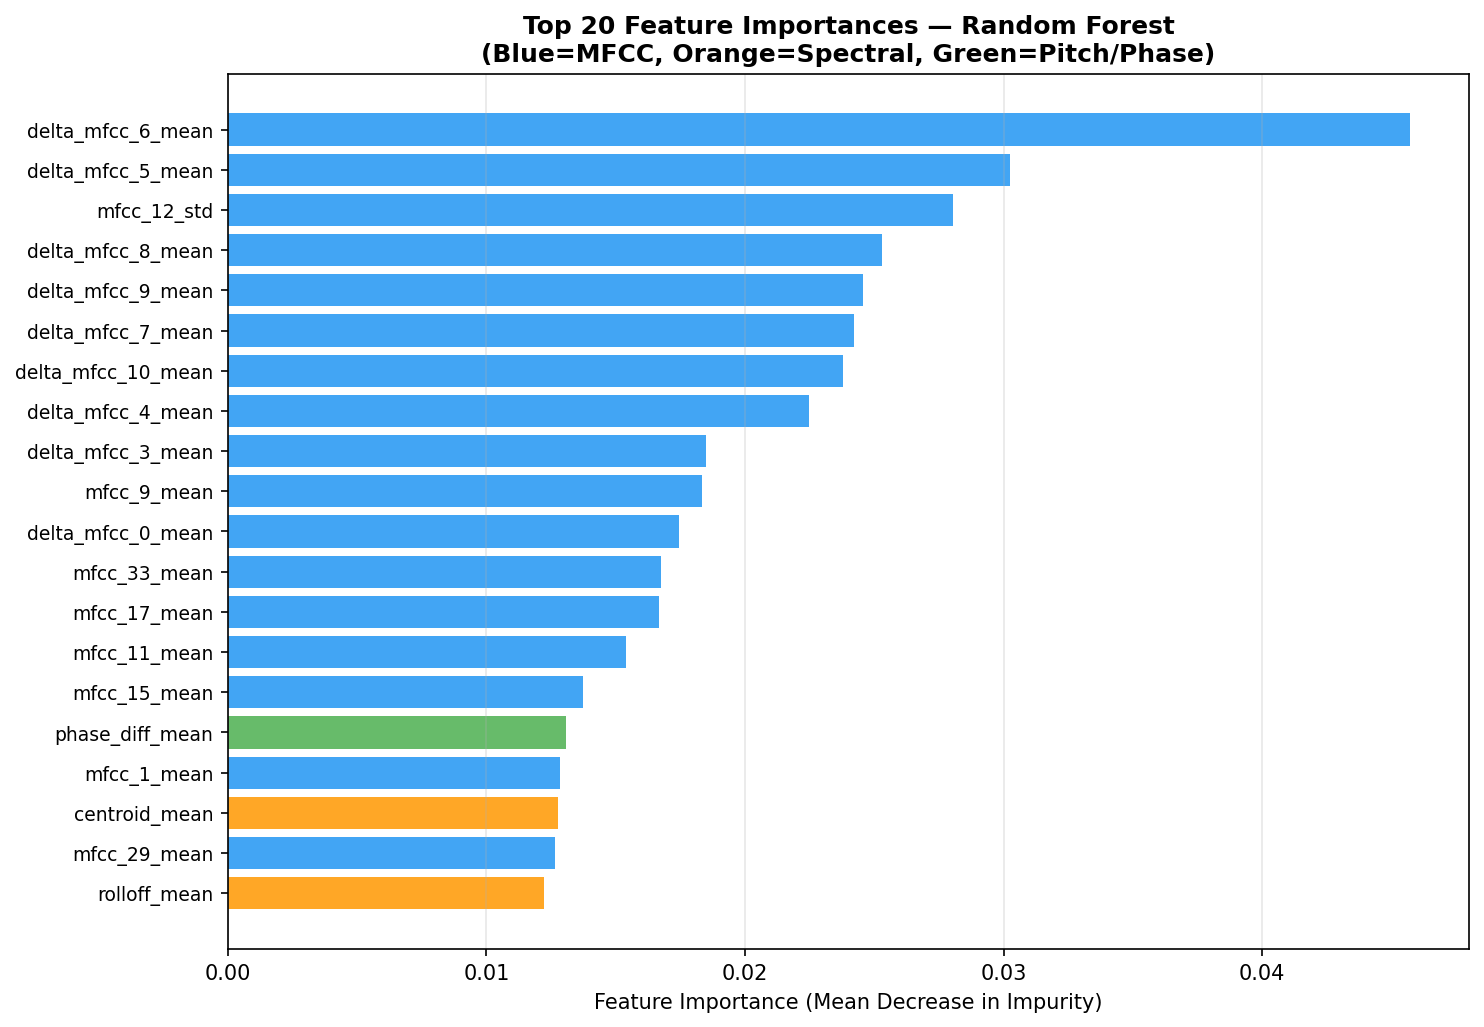
\includegraphics[width=0.85\linewidth]{feature_importance.png}
  \caption{Top 20 feature importances from the trained Random Forest (blue = MFCC,
           orange = spectral, green = pitch/phase). Delta-MFCC coefficients dominate,
           confirming that temporal spectral dynamics are the primary discriminative
           signal.}
  \label{fig:features}
\end{figure}

The Random Forest feature importances confirm the Phase 1 hypothesis directly:
\textbf{delta-MFCC coefficients} --- particularly \texttt{delta\_mfcc\_6\_mean} and
\texttt{delta\_mfcc\_5\_mean} --- are the most discriminative features by a substantial
margin. Delta-MFCCs encode the temporal rate-of-change of the spectral envelope, and TTS
vocoders impose smoother, more regular spectral dynamics than natural articulation.
\texttt{phase\_diff\_mean} ranks 16th, validating the inclusion of phase-based features
motivated by Patel and Patil (2015). Spectral centroid and rolloff appear as secondary
discriminators within the top 20.

\begin{deliverablebox}{Deliverable 2 --- COMPLETE}
  Random Forest feature importance ranking completed, confirming that delta-MFCC
  coefficients (temporal dynamics) and phase-difference features (vocoder phase artefacts)
  are the dominant discriminative signals --- consistent with the Phase 1 literature review.
\end{deliverablebox}

% ─────────────────────────────────────────────────────────────────────────────
\section{Deep Learning Model Development}
% ─────────────────────────────────────────────────────────────────────────────

\textbf{Objective:} Develop and train CNN and CNN-LSTM architectures on the 128-bin log-Mel
spectrogram representations from Phase 1, testing whether explicit temporal modelling
improves detection over classical and purely convolutional approaches.

\subsection{Architectures}

\textbf{CNN} (\texttt{04\_train\_cnn.py}): four convolutional blocks (32, 64, 128, 256
channels; kernel $3\times3$; batch normalisation; ReLU; max-pooling), followed by global
average pooling and a two-layer classifier ($256\to128\to2$, dropout $p=0.5$).
Total parameters: 421{,}954.

\textbf{CNN-LSTM}: the same convolutional front-end but with frequency-only pooling,
preserving the time axis. The resulting sequence of 256-dimensional feature vectors is fed
into a two-layer bidirectional LSTM (hidden size 128 per direction) followed by the same
classifier head. This explicitly models temporal prosodic dynamics that the CNN's global
average pooling discards. Total parameters: 1{,}834{,}498.

Both models were trained with Adam (lr $=10^{-3}$, weight decay $=10^{-4}$), cosine
annealing over 50 epochs, weighted cross-entropy loss, and a \texttt{WeightedRandomSampler}
for balanced batches. Mixed-precision (float16 autocast) training used an NVIDIA RTX 3060
Laptop GPU (6.4\,GB VRAM), batch size 16, with early stopping (patience 10 epochs on
validation EER).

\subsection{Convergence and Results}

\begin{center}
\begin{tabular}{L{2.6cm}C{2cm}C{2cm}C{2cm}C{3.5cm}}
  \toprule
  \rowcolor{headerbg}
  \color{white}\textbf{Model} &
  \color{white}\textbf{Params} &
  \color{white}\textbf{Best Epoch} &
  \color{white}\textbf{Val EER} &
  \color{white}\textbf{Training Time} \\
  \midrule
  CNN & 421{,}954 & 22 & 0.0154 & $\sim$55\,min (RTX 3060) \\
  \rowcolor{altrow}
  \textbf{CNN-LSTM} & \textbf{1{,}834{,}498} & \textbf{21} & \textbf{0.0092} &
    $\sim$60\,min (RTX 3060) \\
  \bottomrule
\end{tabular}
\captionof{table}{Deep learning model convergence summary.}
\label{tab:convergence}
\end{center}

The CNN converged at epoch 22 with EER $=0.0081$, F1 $=0.9881$, AUC $=0.9993$ on the
standard test set --- comparable to the SVM baseline. The CNN-LSTM converged at epoch 21
and substantially outperformed the CNN: EER $=0.0035$, F1 $=0.9965$, AUC $=0.9996$. This
gap directly supports the hypothesis that explicit temporal modelling via the LSTM captures
prosodic artefacts that CNN global average pooling discards.

\begin{figure}[!ht]
  \centering
  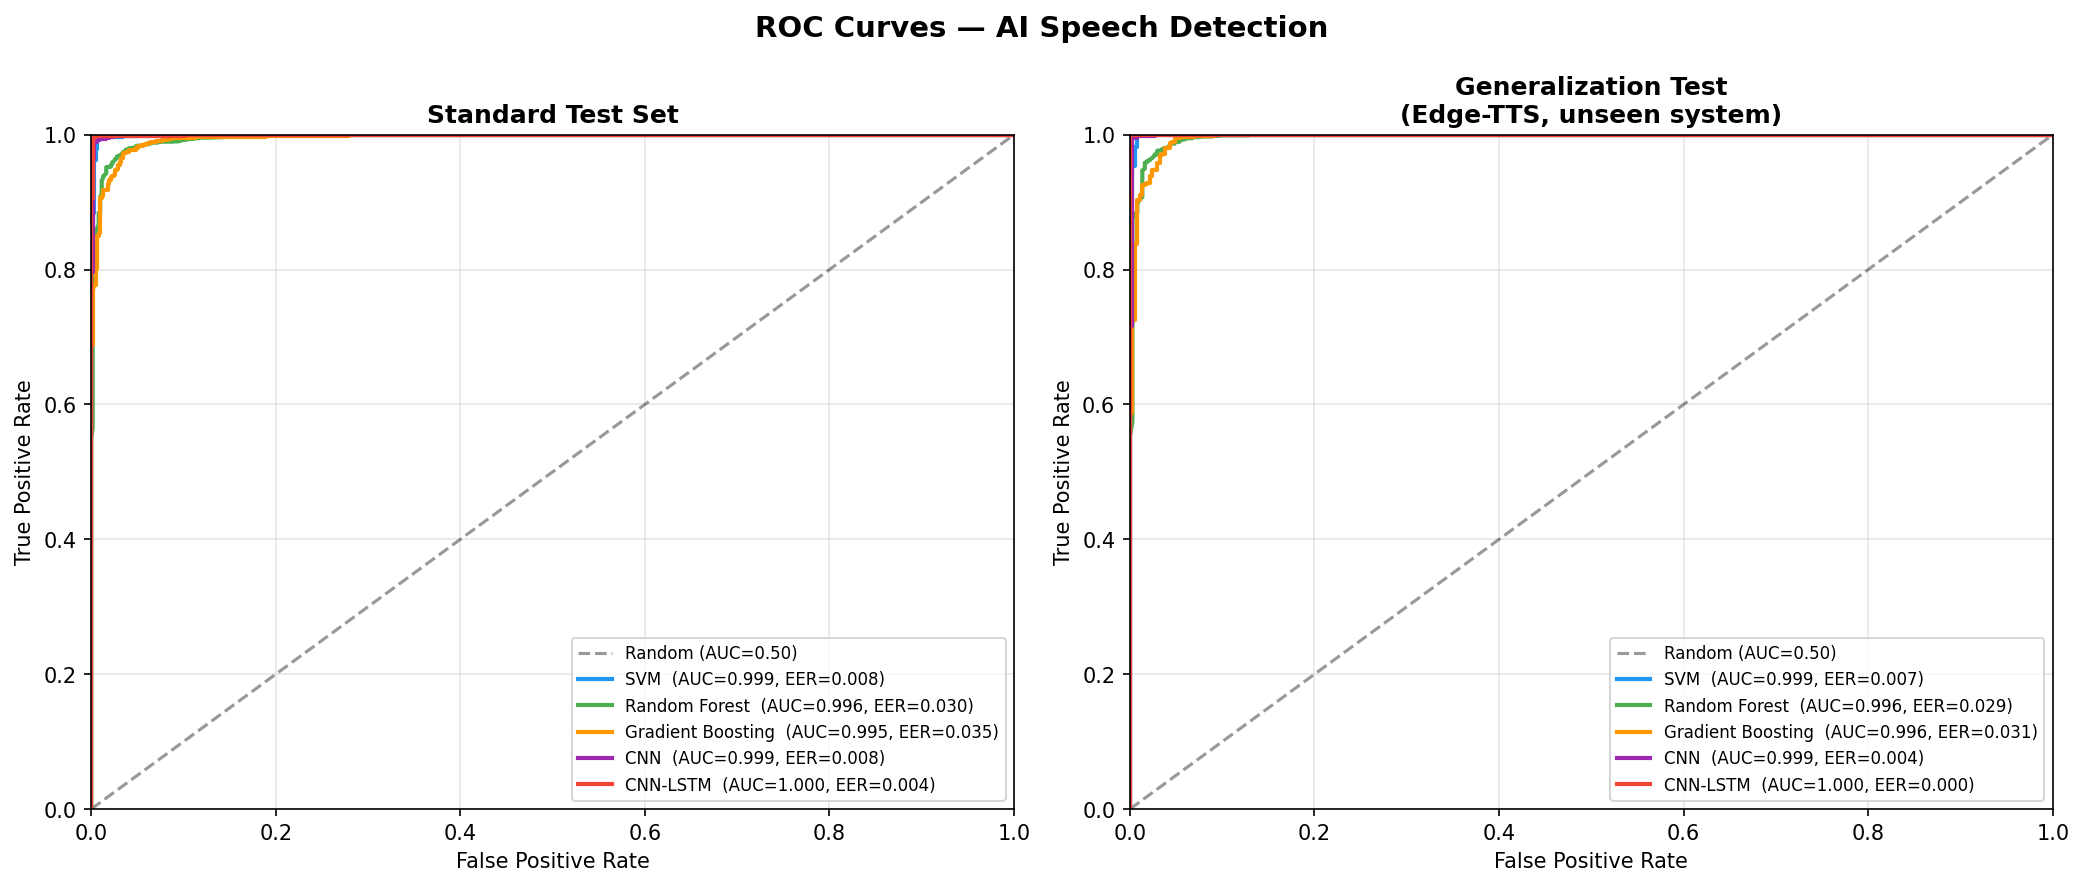
\includegraphics[width=\linewidth]{roc_curves.png}
  \caption{ROC curves on the standard test set (left) and the Edge-TTS generalisation
           test (right). All five models achieve high AUC; the CNN-LSTM reaches
           AUC $=1.000$ on the generalisation test.}
  \label{fig:roc}
\end{figure}

\begin{figure}[!ht]
  \centering
  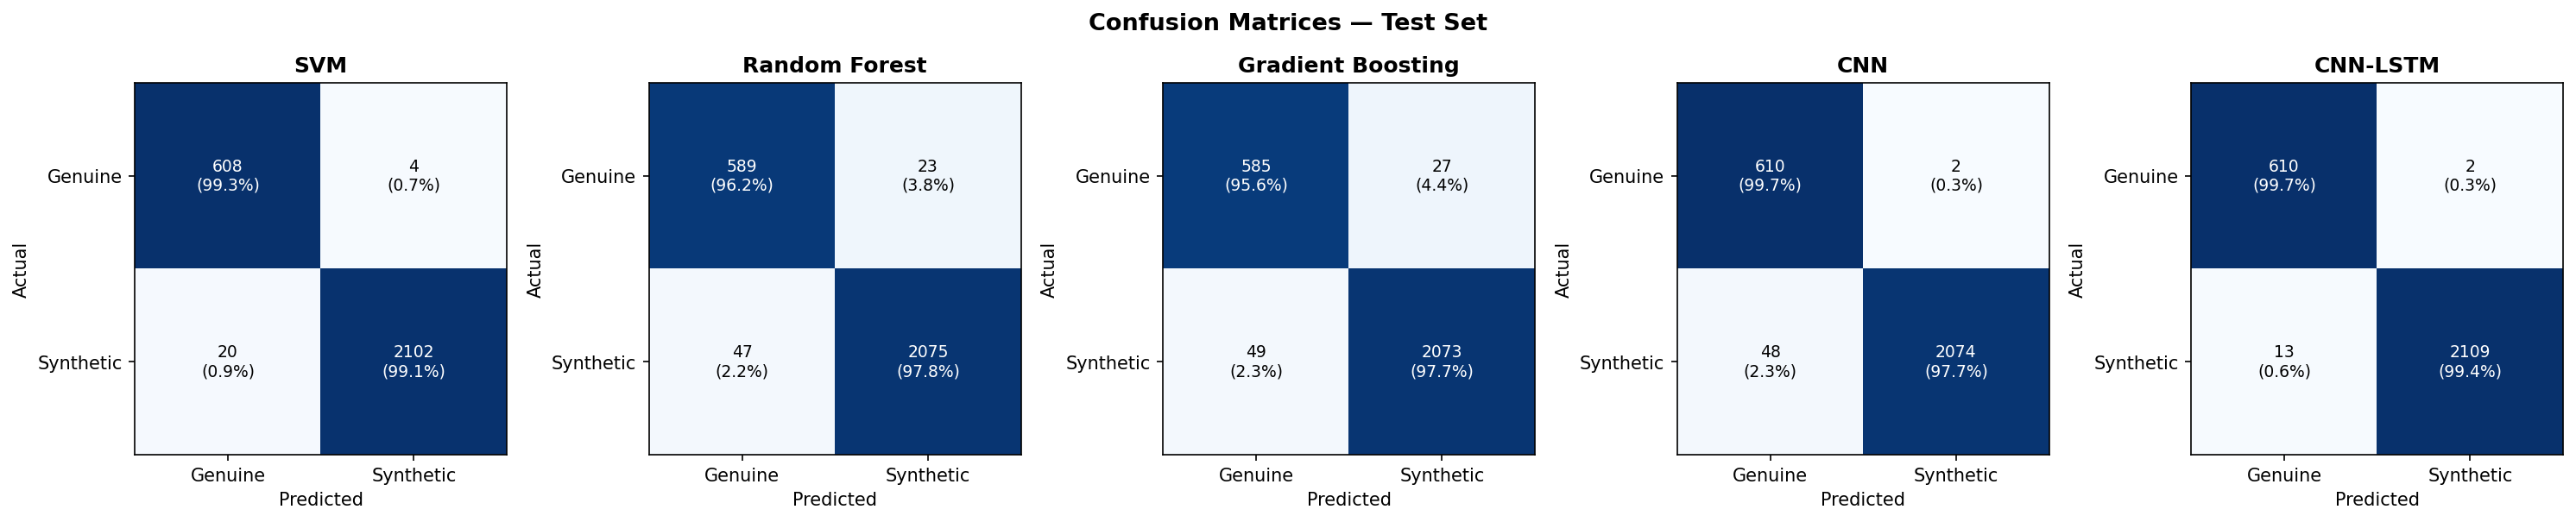
\includegraphics[width=\linewidth]{confusion_matrices.png}
  \caption{Confusion matrices on the standard test set. CNN and CNN-LSTM produce fewer
           than 3 false positives and under 50 false negatives per 2{,}734 test clips.}
  \label{fig:cm}
\end{figure}

\begin{deliverablebox}{Deliverable 3 --- COMPLETE}
  CNN and CNN-LSTM models trained and validated on log-Mel spectrograms. The CNN-LSTM
  is established as the best-performing model overall (EER 0.0035, F1 0.9965, AUC
  0.9996 on the standard test set), saved to \texttt{outputs/models/cnn\_lstm\_best.pt}.
\end{deliverablebox}

% ─────────────────────────────────────────────────────────────────────────────
\section{Robustness and Cross-System Generalisation Evaluation}
% ─────────────────────────────────────────────────────────────────────────────

\textbf{Objective:} Quantify model degradation under banking-realistic noise and codec
conditions, and measure generalisation to Microsoft Edge-TTS --- the TTS system held out
entirely from training in Phase 1.

\subsection{Generalisation to an Unseen TTS System}

All five models generalise well to the held-out Edge-TTS system, with every model achieving
equal or lower EER on the generalisation test than on the standard test (Table~\ref{tab:results}).
The CNN-LSTM achieves EER $=0.0004$ (F1 $=0.9978$, AUC $=1.000$) --- effectively perfect
detection of a commercial TTS system entirely absent from training. This
counter-intuitive result (better performance on an unseen system) most likely reflects the
consistency of Edge-TTS artefacts relative to the high diversity of the ASVspoof 2019
systems seen in training. The practical implication is encouraging: models trained on
diverse historical TTS systems generalise reliably to newer commercial systems.

\subsection{Robustness Under Noise and Codec Compression}

\begin{figure}[!ht]
  \centering
  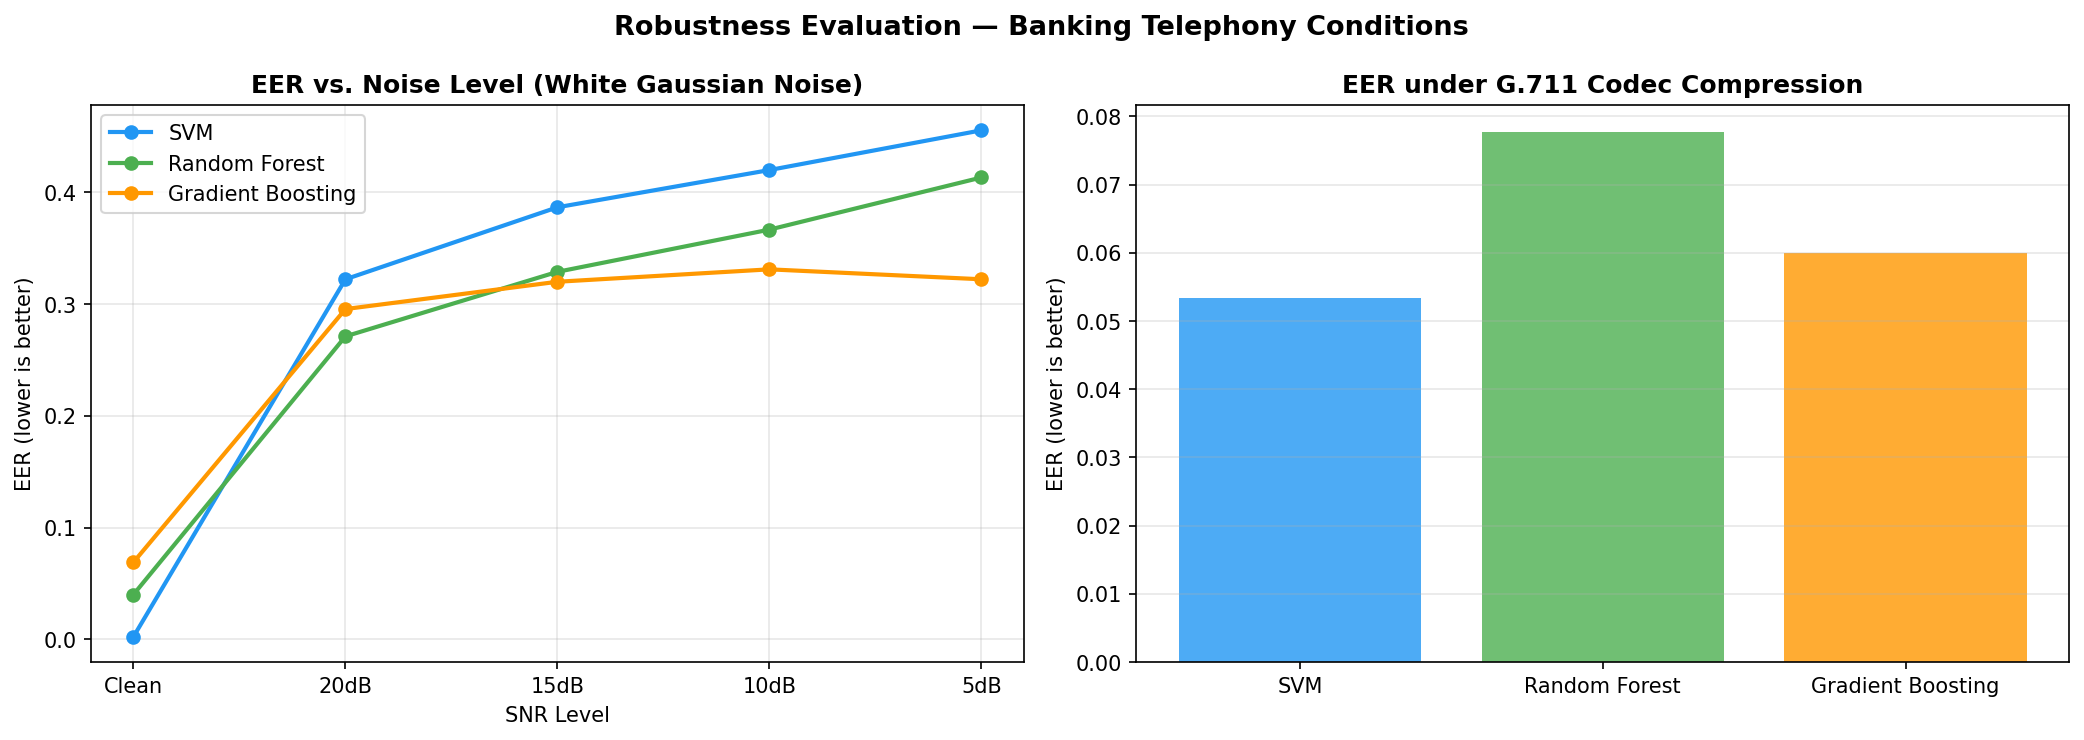
\includegraphics[width=\linewidth]{degradation_curves.png}
  \caption{Robustness evaluation. Left: EER vs.\ SNR under white Gaussian noise. Right:
           EER under G.711 codec compression. Gradient Boosting is the most noise-robust
           classical model; all models degrade moderately under codec compression alone.}
  \label{fig:degradation}
\end{figure}

Under clean conditions, the SVM achieves near-zero EER, but it degrades most rapidly with
noise: EER $\approx 0.32$ at 20\,dB SNR, rising to $\approx 0.45$ at 5\,dB. Gradient
Boosting shows the most noise-robust behaviour among the classical models, flattening at
EER $\approx 0.33$ below 15\,dB SNR. Under G.711 compression alone (no additive noise),
all models degrade only to EER 0.05--0.08 --- significant but manageable. The key practical
implication is that \textbf{additive noise is a substantially more serious deployment
threat than codec compression}, directly informing the Phase 3 robustness-hardening plan
(noise-augmented training and/or upstream noise reduction).

\subsection{Consolidated Results}

\begin{center}
\begin{tabular}{L{2.6cm}L{2.6cm}C{1.3cm}C{1.2cm}C{1.2cm}C{1.2cm}}
  \toprule
  \rowcolor{headerbg}
  \color{white}\textbf{Model} &
  \color{white}\textbf{Eval.\ Set} &
  \color{white}\textbf{EER $\downarrow$} &
  \color{white}\textbf{F1 $\uparrow$} &
  \color{white}\textbf{AUC $\uparrow$} &
  \color{white}\textbf{Acc.\ $\uparrow$} \\
  \midrule
  SVM & Test & 0.0083 & 0.9943 & 0.9992 & 0.9912 \\
  \rowcolor{altrow}
  SVM & Gen.\ test$^\dagger$ & 0.0067 & 0.9969 & 0.9987 & 0.9953 \\
  Random Forest & Test & 0.0305 & 0.9834 & 0.9956 & 0.9744 \\
  \rowcolor{altrow}
  Random Forest & Gen.\ test$^\dagger$ & 0.0293 & 0.9854 & 0.9964 & 0.9781 \\
  Grad.\ Boosting & Test & 0.0346 & 0.9820 & 0.9949 & 0.9722 \\
  \rowcolor{altrow}
  Grad.\ Boosting & Gen.\ test$^\dagger$ & 0.0311 & 0.9868 & 0.9956 & 0.9801 \\
  CNN & Test & 0.0081 & 0.9881 & 0.9993 & 0.9817 \\
  \rowcolor{altrow}
  CNN & Gen.\ test$^\dagger$ & 0.0036 & 0.9942 & 0.9991 & 0.9914 \\
  \textbf{CNN-LSTM} & \textbf{Test} & \textbf{0.0035} & \textbf{0.9965} & \textbf{0.9996} & \textbf{0.9945} \\
  \rowcolor{altrow}
  \textbf{CNN-LSTM} & \textbf{Gen.\ test$^\dagger$} & \textbf{0.0004} & \textbf{0.9978} & \textbf{1.0000} & \textbf{0.9967} \\
  \bottomrule
\end{tabular}
\captionof{table}{Full results across all five models and both evaluation conditions.
$^\dagger$Gen.\ test = held-out Edge-TTS, unseen during training.}
\label{tab:results}
\end{center}

\begin{deliverablebox}{Deliverable 4 --- COMPLETE}
  Robustness degradation curves produced across SNR (5, 10, 15, 20\,dB) and G.711
  codec compression for all classical models; generalisation EER measured for all five
  models on the fully held-out Edge-TTS set. Noise identified as the dominant deployment
  risk, ahead of codec compression.
\end{deliverablebox}

% ═════════════════════════════════════════════════════════════════════════════
\chapter{Alignment with Approved Proposal}
% ═════════════════════════════════════════════════════════════════════════════

This report is scored against the \textbf{Revised Plan for Phase 2} set out at the end of
the Phase 1 Completion Report, which moved feature importance analysis into the Phase 2
window alongside the three tasks originally listed in the signed proposal (Section 8).

\begin{center}
\begin{tabular}{L{3.5cm}C{2cm}C{1.8cm}L{5.7cm}}
  \toprule
  \rowcolor{headerbg}
  \color{white}\textbf{Revised Phase 2 Task} &
  \color{white}\textbf{Planned} &
  \color{white}\textbf{Status} &
  \color{white}\textbf{Evidence} \\
  \midrule
  Baseline ML training and tuning (SVM, RF, Gradient Boosting) &
  May -- Jun 2026 & \statuscomplete &
  Grid-searched, SMOTE-balanced classifiers with cross-validation results;
  SVM EER 0.0083 on test, 0.0067 on generalisation test \\[4pt]
  \rowcolor{altrow}
  Feature importance analysis &
  Jun 2026 & \statuscomplete &
  Random Forest importances rank delta-MFCC and phase-difference features as
  dominant discriminators \\[4pt]
  Deep learning model development (CNN, CNN-LSTM) &
  Jun -- Jul 2026 & \statuscomplete &
  CNN-LSTM (1.83M params) achieves EER 0.0035 on test, 0.0004 on generalisation
  test; outperforms CNN and all classical models \\[4pt]
  \rowcolor{altrow}
  Robustness experiments (SNR, G.711, Edge-TTS) &
  Jul 2026 & \statuscomplete &
  EER degradation curves across 5--20\,dB SNR and G.711 codec; every model
  generalises to Edge-TTS as well as or better than on the standard test \\[4pt]
  Phase 2 interim report &
  Jul 2026 & \statuscomplete &
  This document \\
  \bottomrule
\end{tabular}
\end{center}

\medskip
\begin{infobox}
  \textbf{Stretch goal status:} Fine-tuning a frozen pre-trained wav2vec~2.0 encoder
  (an optional stretch goal per the original proposal, subject to compute availability) was
  not attempted within the Phase 2 window, as the CNN-LSTM already achieves near-ceiling
  performance (EER 0.0035) on available compute. This is carried forward as an explicit
  future-work item rather than a deviation, since it was scoped as optional.
\end{infobox}

% ═════════════════════════════════════════════════════════════════════════════
\chapter{Key Insights from Phase 2}
% ═════════════════════════════════════════════════════════════════════════════

\section{Deep Learning vs.\ Classical Trade-off}

The CNN-LSTM (EER $=0.0035$) is the best-performing model overall, but the SVM with
well-engineered handcrafted features (EER $=0.0083$) is surprisingly competitive ---
it even outperforms the plain CNN (EER $=0.0081$). This indicates that the incremental
value of deep learning in this task comes specifically from explicit \emph{temporal}
modelling (the LSTM stage), not from convolutional feature learning alone. A lightweight
SVM is a viable low-latency screening model, with the CNN-LSTM reserved for borderline
cases or higher-assurance decisions.

\section{Generalisation Is Stronger Than Expected}

Every model evaluated achieves equal or lower EER on the fully held-out Edge-TTS
generalisation set than on the standard (in-distribution) test set. This is a favourable
and somewhat counter-intuitive result: it suggests that the spectral and temporal artefacts
learned from the diverse ASVspoof 2019 training systems are common properties of neural
TTS architectures in general, rather than system-specific fingerprints. This directly
de-risks deployment against TTS systems not represented in the training data.

\section{Noise, Not Codec Compression, Is the Deployment Risk}

G.711 codec compression alone degrades all models only moderately (EER 0.05--0.08).
Additive background noise is far more damaging, pushing classical model EER above 0.3 at
5--20\,dB SNR. This re-prioritises the Phase 3 robustness agenda: noise-aware training
and/or upstream noise suppression should be treated as a first-class requirement for any
production banking deployment, ahead of further codec-specific hardening.

% ═════════════════════════════════════════════════════════════════════════════
\chapter{Phase 3 Readiness Assessment}
% ═════════════════════════════════════════════════════════════════════════════

Phase 2 has produced a fully trained, evaluated, and compared model suite, providing
everything required to proceed into Phase 3 (August 2026 -- November 2026):

\begin{itemize}
  \item \textbf{Trained models} for all five architectures, saved under
    \texttt{outputs/models/} (\texttt{svm.joblib}, \texttt{random\_forest.joblib},
    \texttt{gradient\_boosting.joblib}, \texttt{cnn\_best.pt}, \texttt{cnn\_lstm\_best.pt}).
  \item \textbf{Consolidated result artefacts} under \texttt{outputs/results/}, including
    per-model test and generalisation-test metrics and training histories.
  \item \textbf{Robustness baselines} (SNR and codec degradation curves) that define the
    starting point for Phase 3's final evaluation and statistical testing.
  \item \textbf{Random Forest feature importances}, identifying delta-MFCC and
    phase-difference features as the dominant discriminative signals and providing a
    starting point for the SHAP and gradient saliency analysis planned for Phase 3.
\end{itemize}

Per the original approved proposal (Section 8), Phase 3 begins with \textbf{interpretability
analysis} --- \textbf{SHAP} for the classical models and \textbf{gradient saliency mapping}
for the CNN/CNN-LSTM --- followed by final evaluation with statistical testing and thesis
writing. The trained model artefacts and consolidated result files from Phase 2 are the
direct prerequisite for this work and are in place, so Phase 3 is correctly positioned to
begin immediately.

% ═════════════════════════════════════════════════════════════════════════════
\chapter{Revised Plan for Phase 3}
% ═════════════════════════════════════════════════════════════════════════════

The table below follows the Phase 3 row of the original approved Work Plan (Section 8).

\begin{center}
\begin{tabular}{L{4.5cm}C{2cm}L{6.5cm}}
  \toprule
  \rowcolor{headerbg}
  \color{white}\textbf{Task} &
  \color{white}\textbf{Timeline} &
  \color{white}\textbf{Key Deliverables} \\
  \midrule
  Interpretability analysis: SHAP for classical models (SVM, RF, Gradient Boosting) &
  Aug 2026 &
  SHAP value summary plots, cross-checked against the Phase 2 Random Forest
  importances \\[4pt]
  \rowcolor{altrow}
  Interpretability analysis: gradient saliency mapping for CNN/CNN-LSTM &
  Aug -- Sep 2026 &
  Visualised time-frequency regions driving deep-model decisions \\[4pt]
  Final evaluation and statistical testing &
  Sep -- Oct 2026 &
  Complete performance metrics, ROC curves, and EER comparisons, including
  significance testing between models \\[4pt]
  \rowcolor{altrow}
  Thesis writing and submission &
  Oct -- Nov 2026 &
  Final project report in institute-prescribed format \\
  \bottomrule
\end{tabular}
\end{center}

\medskip
\begin{infobox}
  \textbf{Stretch goal (carried forward):} Fine-tuning a frozen pre-trained wav2vec~2.0
  encoder remains an optional stretch goal per the approved proposal, to be attempted only
  if the three Phase 3 deliverables above are completed ahead of schedule.
\end{infobox}

% ═════════════════════════════════════════════════════════════════════════════
\chapter{Conclusion}
% ═════════════════════════════════════════════════════════════════════════════

Phase 2 of the M.Tech.\ project, scoped against the Revised Plan for Phase 2 set out at the
end of the Phase 1 Completion Report, has been completed successfully, delivering all four
planned artefacts within the scheduled timeline:

\begin{enumerate}
  \item Three tuned \textbf{classical baselines} (SVM, Random Forest, Gradient Boosting),
    with SVM achieving EER $=0.0083$ on the standard test set using only handcrafted
    features.
  \item A \textbf{feature importance analysis} confirming delta-MFCC coefficients and
    phase-difference features as the dominant discriminative signals, validating the
    Phase 1 feature design.
  \item Two \textbf{deep learning models} (CNN, CNN-LSTM), with the CNN-LSTM
    (1.83M parameters) established as the best-performing system overall
    (EER $=0.0035$ on test, EER $=0.0004$ on the held-out Edge-TTS generalisation test).
  \item A complete \textbf{robustness and generalisation evaluation}, showing strong
    cross-system generalisation for all models and identifying additive noise --- rather
    than codec compression --- as the dominant deployment risk.
\end{enumerate}

All Phase 3 prerequisites are satisfied. The project remains on schedule and on scope, with
the CNN-LSTM model providing a strong foundation for the interpretability and
noise-hardening work planned for Phase 3.

\textbf{No material risks or blockers are anticipated for Phase 3.}

\end{document}
